% Provenance (never printed): see sources/outline_sources.md (Year 3: the heat
% equation, half-space and plate cooling models, heat flow against age,
% continental geotherms, thermal subsidence). Brief: sources/book5/BRIEFS.md,
% ch. 5. Curves from figdata/bachelor-3/plate_cooling.py (models; Seton et al.
% 2020 age grid and ETOPO1, read only) and continental_geotherm.py.
% Exercise and problem values in the Book 5 scratch calculator calc/ch05.py.
\chapter{Modèles thermiques de la lithosphère}\label{ch:b3:lithosphere-thermal-models}

Il suffit de s'éloigner d'une dorsale médio-océanique pour que le fond marin s'approfondisse~: environ
\qty{2.5}{km} à l'axe, et plus de \qty{5}{km} sous le plancher océanique le plus ancien.
Rien n'a été ajouté à la plaque ni retiré~: elle a seulement
refroidi, s'est contractée et enfoncée. Le plancher océanique est un thermomètre de la plaque
située sous lui, et une sonde de flux de chaleur enfoncée dans ses sédiments lit le même
refroidissement, vu d'en haut. Ce chapitre résout de deux façons le refroidissement d'une plaque,
en demi-espace et en plaque d'épaisseur finie, compare les deux solutions à la profondeur
réelle du fond océanique et à son flux de chaleur, puis s'intéresse aux continents,
dont une partie de la chaleur provient de leur propre croûte.
% ledger: ps77:depth-age

\begin{recall}
L'équation de diffusion de la chaleur, $\partial T/\partial t = \kappa\nabla^2T$,
avec la conductivité thermique $k$ et la diffusivité thermique $\kappa =
k/(\rho c)$, est donnée dans les volumes de physique~; les séries de Fourier et la fonction d'erreur
$\operatorname{erf}x = (2/\sqrt\pi)\int_0^xe^{-u^2}\,\mathrm du$ sont dans les
volumes universitaires de mathématiques. Le flux de chaleur, la production de chaleur
radiogénique, le géotherme, le temps caractéristique conductif $L^2/\kappa$, la
couche limite thermique et la lithosphère thermique ont été définis dans le volume de première année,
dans son chapitre sur le bilan thermique de la Terre~; l'isostasie dans son chapitre
sur l'isostasie et les anomalies de gravité~; la loi profondeur--âge $d = d_r + C\sqrt t$ a été
démontrée dans son chapitre sur les rifts, les dorsales et les marges passives, en admettant le
profil de température que ce chapitre établit. Le modèle d'étirement des bassins, la
subsidence post-rift et la constante de temps thermique figurent dans le volume de deuxième année, dans son
chapitre sur les bassins sédimentaires.
\end{recall}

\section{Conduction, advection et leur rapport}

La chaleur se déplace dans la lithosphère de deux manières~: elle diffuse le long du gradient
de température, et elle est transportée par la roche en mouvement, la plaque quittant une dorsale, une
montagne érodée qui se soulève, un magma qui remonte. Lequel des deux l'emporte dépend d'un seul
nombre.

\begin{definition}[Nombre de Péclet thermique]\label{def:b3:lithosphere-thermal-models:peclet}
Pour une roche se déplaçant à la vitesse $u$ sur une longueur $L$, le \emph{nombre de Péclet
thermique}\index{nombre de Péclet thermique} est
\[
  \mathrm{Pe} = \frac{uL}{\kappa},
\]
le rapport entre le temps conductif $L^2/\kappa$ et le temps advectif $L/u$.
L'advection domine là où $\mathrm{Pe} \gg 1$, la conduction là où
$\mathrm{Pe} \ll 1$.
\end{definition}

Une plaque qui quitte une dorsale à \qty{25}{mm/an} présente, sur une distance de
\qty{95}{km}, $\mathrm{Pe} \approx 94$ avec $\kappa = \qty{0.8e-6}{m^2.s^{-1}}$~:
la chaleur est transportée latéralement par la plaque bien plus vite qu'elle ne diffuse latéralement.
Chaque colonne verticale de la plaque se refroidit donc comme si elle était seule, par
conduction verticale vers le fond marin froid, son âge $t$ désignant le temps écoulé depuis
qu'elle a quitté l'axe. Cela ramène un problème à deux dimensions à un problème en
profondeur et en temps.

\section{Le demi-espace en refroidissement}

\begin{definition}[Modèle de refroidissement du demi-espace]\label{def:b3:lithosphere-thermal-models:half-space}
Le \emph{modèle de refroidissement du demi-espace}\index{modèle de refroidissement du demi-espace} de la
lithosphère océanique assimile chaque colonne à un demi-espace $z \ge 0$ de diffusivité
uniforme, à la température uniforme $T_m$ du manteau lorsqu'elle quitte l'axe de la
dorsale, dont la surface est maintenue dès lors à la température $T_0$ du fond marin,
sans production de chaleur et sans base.
\end{definition}

\begin{theorem}[Géotherme en fonction d'erreur]\label{thm:b3:lithosphere-thermal-models:erf}
Dans le \omterm{def:b3:lithosphere-thermal-models:half-space}{modèle de refroidissement du demi-espace}, la température à la profondeur $z$ sous le
fond marin d'âge $t$ est
\[
  T(z, t) = T_0 + (T_m - T_0)\operatorname{erf}\frac{z}{2\sqrt{\kappa t}} .
\]
C'est le \emph{géotherme en fonction d'erreur}\index{géotherme en fonction d'erreur}.
\end{theorem}

\begin{proof}
Posons $\theta = (T - T_0)/(T_m - T_0)$~; il vérifie $\partial\theta/\partial t =
\kappa\,\partial^2\theta/\partial z^2$ avec $\theta(z, 0) = 1$ pour $z > 0$ et
$\theta(0, t) = 0$ pour $t > 0$. Le problème n'a pas d'échelle de longueur propre~:
si $\theta(z, t)$ est une solution, il en est de même de $\theta(\lambda z, \lambda^2t)$ pour tout
$\lambda > 0$, avec les mêmes conditions initiale et aux limites~; la solution étant
unique, $\theta$ ne dépend de $z$ et $t$ qu'à travers $\eta = z/(2\sqrt{\kappa
t})$. En écrivant $\theta = f(\eta)$, avec $\partial\eta/\partial t = -\eta/(2t)$ et
$\partial\eta/\partial z = 1/(2\sqrt{\kappa t})$,
\[
  -\frac{\eta}{2t}f'(\eta) = \kappa\,\frac{f''(\eta)}{4\kappa t},
  \qquad\text{donc}\qquad f'' + 2\eta f' = 0 .
\]
Donc $f' = Ae^{-\eta^2}$ et $f = A\int_0^\eta e^{-u^2}\,\mathrm du + B$. La
condition en surface, en $\eta = 0$, donne $B = 0$~; la condition initiale, qui
vaut à toute profondeur lorsque $t \to 0$, soit lorsque $\eta \to \infty$, donne
$A\sqrt\pi/2 = 1$. Donc $f = \operatorname{erf}\eta$.
\end{proof}

À profondeur donnée, la température ne dépend que de $z/\sqrt t$~: une isotherme s'enfonce
comme la racine carrée de l'âge, et la couche refroidie à \qty{40}{Ma} est deux fois
plus épaisse qu'à \qty{10}{Ma}. Le flux de chaleur en surface s'en déduit par dérivation.

\begin{proposition}[Relation flux de chaleur--âge]\label{prop:b3:lithosphere-thermal-models:heat-flow}
Dans le \omterm{def:b3:lithosphere-thermal-models:half-space}{modèle de refroidissement du demi-espace}, le flux de chaleur traversant le fond marin d'âge $t$
est
\[
  q(t) = k\,\frac{\partial T}{\partial z}\Big|_{z=0}
  = \frac{k(T_m - T_0)}{\sqrt{\pi\kappa t}} = \frac{C_q}{\sqrt t} .
\]
\end{proposition}

\begin{proof}
$\partial\operatorname{erf}(z/2\sqrt{\kappa t})/\partial z = (2/\sqrt\pi)
e^{-z^2/4\kappa t}/(2\sqrt{\kappa t})$, qui en $z = 0$ vaut $1/\sqrt{\pi\kappa
t}$.
\end{proof}

Avec les valeurs du modèle de plaque ci-dessous ($k = \qty{3.1}{W.m^{-1}.K^{-1}}$,
$T_m - T_0 = \qty{1450}{K}$, $\kappa = \qty{0.8e-6}{m^2.s^{-1}}$), $C_q =
\qty{505}{mW.m^{-2}.Ma^{1/2}}$, proche des valeurs de 430 à
\qty{510}{mW.m^{-2}.Ma^{1/2}} ajustées aux mesures globales par différentes
études~; une compilation récente préfère \num{490}. Le flux de chaleur mesuré sur
la croûte océanique jeune sous-estime toutefois fortement la chaleur qui s'en échappe~:
l'eau de mer qui circule dans la croûte fissurée emporte une partie de la chaleur
vers les sources chaudes, hors de portée des sondes. Sur la croûte ancienne, les mesures
suivent $1/\sqrt t$, et les estimations de la perte de chaleur de la Terre remplacent les
mesures sur la croûte plus jeune que \qty{66.5}{Ma} par $C_q/\sqrt t$.
% ledger: honda04:gdh1, b2dd10:half-space, dd10b5:hydrothermal

Le volume de première année a intégré le même profil sur la profondeur, par
l'isostasie, pour obtenir la loi profondeur--âge, $d = d_r + C\sqrt t$ avec $C = 2\rho_m\alpha(T_m -
T_0)\sqrt\kappa/\bigl(\sqrt\pi(\rho_m - \rho_w)\bigr)$ (figure ci-dessous). Avec
$\rho_m = \qty{3300}{kg.m^{-3}}$, $\rho_w = \qty{1030}{kg.m^{-3}}$ et $\alpha =
\qty{3.1e-5}{K^{-1}}$, $C = \qty{370}{m.Ma^{-1/2}}$, à comparer aux
\qty{350}{m.Ma^{-1/2}} ajustés aux fonds du Pacifique Nord et de l'Atlantique Nord
plus jeunes que \qty{70}{Ma}.
% ledger: ps77:depth-age

\begin{omfigure}
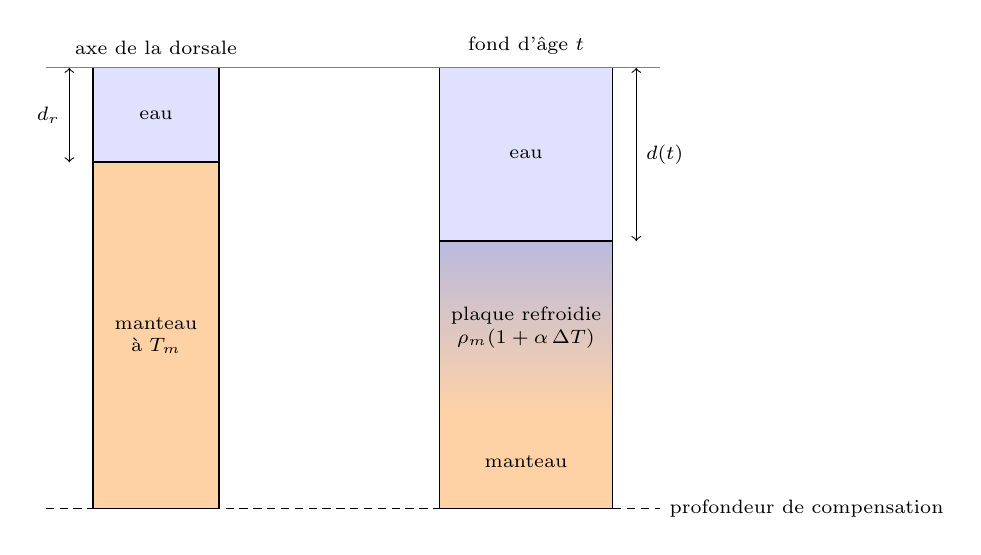
\begin{tikzpicture}[font=\small, x=1cm, y=1cm]
% schematic: two columns of equal mass above the compensation depth
\fill[blue!12] (0,0) rectangle (1.6,-1.2);
\fill[orange!35] (0,-1.2) rectangle (1.6,-5.6);
\fill[blue!12] (4.4,0) rectangle (6.6,-2.2);
\shade[top color=blue!35!gray!40, bottom color=orange!35] (4.4,-2.2) rectangle (6.6,-4.4);
\fill[orange!35] (4.4,-4.4) rectangle (6.6,-5.6);
\draw (0,0) rectangle (1.6,-5.6) (4.4,0) rectangle (6.6,-5.6);
\draw[densely dashed] (-0.6,-5.6) -- (7.2,-5.6) node[right, font=\scriptsize] {profondeur de compensation};
\draw[thick] (0,-1.2) -- (1.6,-1.2) (4.4,-2.2) -- (6.6,-2.2);
\node[font=\scriptsize] at (0.8,-0.6) {eau};
\node[font=\scriptsize, align=center] at (0.8,-3.4) {manteau\\à $T_m$};
\node[font=\scriptsize] at (5.5,-1.1) {eau};
\node[font=\scriptsize, align=center] at (5.5,-3.3) {plaque refroidie\\$\rho_m(1 + \alpha\,\Delta T)$};
\node[font=\scriptsize, align=center] at (5.5,-5.0) {manteau};
\draw[<->] (-0.3,0) -- (-0.3,-1.2) node[midway, left, font=\scriptsize] {$d_r$};
\draw[<->] (6.9,0) -- (6.9,-2.2) node[midway, right, font=\scriptsize] {$d(t)$};
\node[above, font=\scriptsize] at (0.8,0.05) {axe de la dorsale};
\node[above, font=\scriptsize] at (5.5,0.05) {fond d'âge $t$};
\draw[gray] (-0.6,0) -- (7.2,0);
\end{tikzpicture}

\par\smallskip{\small Isostasie de la plaque en refroidissement~: la colonne à la dorsale
et la colonne d'âge $t$ ont la même masse au-dessus de la profondeur de compensation. La
plaque refroidie, plus dense, s'enfonce, et l'eau remplit l'espace au-dessus
d'elle.}\label{fig:b3:lithosphere-thermal-models:columns}
\end{omfigure}

\section{Le modèle de plaque}

Le fond océanique ancien cesse de s'approfondir~: dans le Pacifique Nord et
l'Atlantique Nord, la profondeur s'écarte de $\sqrt t$ entre 60 et \qty{80}{Ma}, et le flux de chaleur se stabilise.
Le demi-espace continue de se refroidir indéfiniment~; il faut quelque chose pour maintenir la base de la
plaque chaude.
% ledger: parsons:plate-model

\begin{definition}[Modèle de refroidissement de plaque]\label{def:b3:lithosphere-thermal-models:plate}
Le \emph{modèle de refroidissement de plaque}\index{modèle de refroidissement de plaque} de la
lithosphère océanique considère chaque colonne comme une couche $0 \le z \le L$ de
diffusivité uniforme, à la température uniforme $T_m$ lorsqu'elle quitte la dorsale, dont
la surface est maintenue à $T_0$ et dont la base est maintenue à $T_m$ dès lors.
\end{definition}

\begin{theorem}[Série de température du modèle de plaque]\label{thm:b3:lithosphere-thermal-models:plate-series}
Dans le \omterm{def:b3:lithosphere-thermal-models:plate}{modèle de refroidissement de plaque}, avec $T_0 = 0$,
\[
  T(z, t) = T_m\Bigl[\frac zL + \frac2\pi\sum_{n=1}^\infty\frac1n
  \sin\frac{n\pi z}{L}\,e^{-n^2t/\tau}\Bigr],\qquad
  \tau = \frac{L^2}{\pi^2\kappa} .
\]
Il s'agit de la \emph{série de température du modèle de plaque}\index{série de température du modèle de plaque}.
\end{theorem}

\begin{proof}
L'état stationnaire, atteint lorsque $t \to \infty$, est le profil linéaire $T_mz/L$.
L'écart $u = T - T_mz/L$ satisfait l'équation de diffusion avec $u = 0$ en
$z = 0$ et $z = L$, et part de $u(z, 0) = T_m(1 - z/L)$. En séparant les
variables, $u = Z(z)\Theta(t)$ donne $Z''/Z = \Theta'/(\kappa\Theta) = -\mu^2$~;
les conditions aux limites conduisent à $Z = \sin(n\pi z/L)$, $\mu = n\pi/L$, et
$\Theta = e^{-n^2\pi^2\kappa t/L^2} = e^{-n^2t/\tau}$. Les valeurs initiales fixent les
coefficients $b_n$ de la série en sinus de $T_m(1 - z/L)$ sur $[0, L]$~:
\[
  b_n = \frac2L\int_0^LT_m\Bigl(1 - \frac zL\Bigr)\sin\frac{n\pi z}{L}\,\mathrm dz
  = \frac{2T_m}{n\pi},
\]
par une intégration par parties. La somme des modes donne la série.
\end{proof}

Chaque mode décroît avec son propre temps, $\tau/n^2$~: les harmoniques supérieures, la
structure fine de l'échelon initial, s'annulent les premières, et après un temps
de l'ordre de $\tau$ seul le premier subsiste. La même séparation des variables donne le
flux de chaleur et, par l'équilibre isostatique de la figure ci-dessus, la profondeur.

\begin{proposition}[Profondeur et flux de chaleur du modèle de plaque]\label{prop:b3:lithosphere-thermal-models:plate-depth}
Dans le \omterm{def:b3:lithosphere-thermal-models:plate}{modèle de refroidissement de plaque}, avec les densités et la dilatation de la
loi profondeur--âge,
\[
  q(t) = \frac{kT_m}{L}\Bigl[1 + 2\sum_{n=1}^\infty e^{-n^2t/\tau}\Bigr],\qquad
  d(t) = d_r + \frac{\rho_m\alpha T_mL}{2(\rho_m - \rho_w)}
  \Bigl[1 - \frac{8}{\pi^2}\sum_{n\ \text{impair}}\frac{e^{-n^2t/\tau}}{n^2}\Bigr].
\]
Lorsque $t \to \infty$, la profondeur tend vers $d_r + \rho_m\alpha T_mL/\bigl(2(\rho_m -
\rho_w)\bigr)$ et le flux de chaleur vers $kT_m/L$, tous deux exponentiellement, avec la
constante de temps $\tau$.
\end{proposition}

\begin{proof}
Dérivons la série en $z = 0$~, $\partial T/\partial z = (T_m/L)[1 +
2\sum e^{-n^2t/\tau}]$. Pour la profondeur, l'équilibre isostatique donne $(\rho_m -
\rho_w)(d - d_r) = \rho_m\alpha\int_0^L(T_m - T)\,\mathrm dz$. La partie linéaire
contribue $T_mL/2$~; chaque mode contribue $-(2T_m/n\pi)e^{-n^2t/\tau}
\int_0^L\sin(n\pi z/L)\,\mathrm dz = -(2T_m/n\pi)(L/n\pi)(1 - \cos n\pi)
e^{-n^2t/\tau}$, qui est nul pour $n$ pair et vaut $-(4T_mL/n^2\pi^2)
e^{-n^2t/\tau}$ pour $n$ impair. En factorisant $T_mL/2$, on obtient le crochet. À $t = 0$,
il s'annule, puisque $\sum_{n\ \text{impair}}1/n^2 = \pi^2/8$.
\end{proof}

Le modèle de plaque qui ajuste le mieux les profondeurs et les flux de chaleur globaux
a une plaque de \qty{95}{km} d'épaisseur, avec une base à \qty{1450}{\celsius}, $\alpha =
\qty{3.1e-5}{K^{-1}}$ et $k = \qty{3.1}{W.m^{-1}.K^{-1}}$, plus mince et plus chaud
que les valeurs antérieures de \qty{125}{km} et \qty{1350}{\celsius}. Avec $\kappa =
\qty{0.8e-6}{m^2.s^{-1}}$, $\tau = \qty{36.2}{Ma}$~; la profondeur se stabilise à
$2500 + 3104 = \qty{5604}{m}$ et le flux de chaleur à \qty{47}{mW.m^{-2}}. Le fond
océanique jeune ne permet pas de départager les deux modèles~: ils diffèrent de moins
d'un mètre à \qty{2}{Ma}, et de \qty{100}{m} à \qty{44}{Ma}. La sismologie donne une
réponse voisine~: les \omterm{def:b3:seismology-imaging:surface-waves}{ondes de Rayleigh} du Pacifique sont mieux ajustées par des
plaques de refroidissement dont l'épaisseur asymptotique est comprise entre 85 et \qty{95}{km}.
% ledger: honda04:gdh1, ps77:depth-age, fischer:lithosphere

\begin{omfigure}
\begin{tikzpicture}
\begin{groupplot}[group style={group size=1 by 2, vertical sep=2.3cm},
  omrecord, width=0.86\linewidth, height=0.42\linewidth, xmin=0, xmax=160,
  xlabel={âge du fond océanique (Ma)}]
\nextgroupplot[omdepth, ylabel={profondeur (km)}, ymin=0, ymax=130,
  title={(a) isothermes, tous les \qty{200}{\celsius}}, title style={font=\small},
  legend style={font=\scriptsize, at={(0.01,0.03)}, anchor=south west}]
% computed in figdata/bachelor-3/plate_cooling.py; ledger: honda04:gdh1
\addplot[omDef, thick] table[x=t, y=hs200] {figdata/out/bachelor-3-plate_cooling-isotherms.dat};
\addlegendentry{demi-espace}
\addplot[red!70!black, thick, densely dashed] table[x=t, y=pl200] {figdata/out/bachelor-3-plate_cooling-isotherms.dat};
\addlegendentry{plaque, $L = \qty{95}{km}$}
\foreach \lev in {400,600,800,1000,1200,1400} {
  \addplot[omDef, thick, forget plot] table[x=t, y=hs\lev] {figdata/out/bachelor-3-plate_cooling-isotherms.dat};
  \addplot[red!70!black, thick, densely dashed, forget plot] table[x=t, y=pl\lev] {figdata/out/bachelor-3-plate_cooling-isotherms.dat};
}
\draw[gray] (axis cs:0,95) -- (axis cs:160,95);
\node[font=\scriptsize, anchor=north] at (axis cs:68,96) {base de la plaque};
\node[font=\scriptsize, fill=white, inner sep=1pt] at (axis cs:150,14) {200};
\node[font=\scriptsize, fill=white, inner sep=1pt] at (axis cs:28,38.2) {1000};
\node[font=\scriptsize, fill=white, inner sep=1pt] at (axis cs:22,70.4) {1400};
\nextgroupplot[ylabel={flux de chaleur (\unit{mW.m^{-2}})}, ymin=0, ymax=300,
  title={(b) flux de chaleur}, title style={font=\small},
  legend style={font=\scriptsize, at={(0.98,0.97)}, anchor=north east}]
\addplot[omDef, thick] table[x=t, y=hs] {figdata/out/bachelor-3-plate_cooling-heat.dat};
\addlegendentry{demi-espace}
\addplot[red!70!black, thick, densely dashed] table[x=t, y=pl] {figdata/out/bachelor-3-plate_cooling-heat.dat};
\addlegendentry{plaque}
\end{groupplot}
\end{tikzpicture}

\par\smallskip{\small Les deux modèles de refroidissement avec les paramètres du texte.
(a) Profondeur des isothermes de \qty{200}{\celsius} (en haut) à
\qty{1400}{\celsius} (en bas)~: celles du demi-espace continuent de s'enfoncer en
$\sqrt t$, celles de la plaque s'arrêtent lorsque le profil devient linéaire. (b) Flux de
chaleur en surface~: le modèle de plaque se stabilise à \qty{47}{mW.m^{-2}}, tandis que
celui du demi-espace décroît en $1/\sqrt t$.}\label{fig:b3:lithosphere-thermal-models:isotherms}
\end{omfigure}

Le fond océanique réel peut être reporté sur le même graphique (figure ci-dessous). Chaque
case d'un degré de latitude et de longitude dont l'âge est connu est placée à son âge et
à sa profondeur~; la médiane de chaque intervalle de cinq millions d'années croît avec
l'âge comme le prévoient les modèles pour les \qty{40}{Ma} initiaux, mais le fond observé
est moins profond que les deux modèles, et de plus en plus à mesure que l'âge augmente. Rien n'a été corrigé~: le vieux fond
porte une couverture sédimentaire plus épaisse, de plus d'un kilomètre dans la partie ancienne
de l'Atlantique Nord, qui le charge et en relève le sommet, et le vieux fond a eu le temps
d'accumuler monts sous-marins, plateaux volcaniques et bourrelets des points chauds. Les ajustements publiés
retirent d'abord la charge sédimentaire et les bourrelets évidents~; la loi profondeur--âge
du volume de première année, ainsi que les modèles de plaque ci-dessus, proviennent de telles
profondeurs corrigées.
% ledger: data:b5-depth-age, ps77:depth-age

\begin{omfigure}
\begin{tikzpicture}
\begin{axis}[omrecord, omdepth, width=0.86\linewidth, height=0.5\linewidth,
  xmin=0, xmax=180, ymin=2, ymax=6.5, xlabel={âge du fond océanique (Ma)},
  ylabel={profondeur (km)},
  legend style={font=\scriptsize, at={(0.5,-0.24)}, anchor=north, cells={anchor=west}},
  legend columns=2]
% computed in figdata/bachelor-3/plate_cooling.py; ledger: data:b5-depth-age, honda04:gdh1
\addplot[only marks, mark=*, mark size=1.3pt, black,
  error bars/.cd, y dir=both, y explicit]
  table[x=t, y expr=\thisrow{med}/1000, y error plus expr=(\thisrow{q3}-\thisrow{med})/1000,
  y error minus expr=(\thisrow{med}-\thisrow{q1})/1000] {figdata/out/bachelor-3-plate_cooling-bins.dat};
\addlegendentry{observé, médiane et quartiles}
\addplot[omDef, thick] table[x=t, y expr=\thisrow{hs}/1000] {figdata/out/bachelor-3-plate_cooling-depth.dat};
\addlegendentry{demi-espace}
\addplot[red!70!black, thick, densely dashed] table[x=t, y expr=\thisrow{pl}/1000] {figdata/out/bachelor-3-plate_cooling-depth.dat};
\addlegendentry{plaque, $L = \qty{95}{km}$}
\end{axis}
\end{tikzpicture}

\par\smallskip{\small Profondeur du fond océanique en fonction de son âge~: la médiane et
les quartiles des profondeurs des cases d'un degré de chaque intervalle de cinq millions
d'années (fond océanique plus profond que \qty{1000}{m}, âges issus d'une grille mondiale
d'âges, profondeurs issues d'un modèle mondial de relief, sans correction pour les
sédiments, les monts sous-marins ou les bourrelets), avec les deux modèles de refroidissement du texte.}\label{fig:b3:lithosphere-thermal-models:depth-age}
\end{omfigure}

\begin{definition}[Subsidence thermique]\label{def:b3:lithosphere-thermal-models:thermal-subsidence}
La \emph{subsidence thermique}\index{subsidence thermique} est l'enfoncement de la
surface de la lithosphère lorsqu'elle se refroidit et se contracte vers l'équilibre
thermique, l'espace situé au-dessus étant comblé par de l'eau ou des sédiments~; l'isostasie
convertit la chaleur perdue par une colonne en son enfoncement.
\end{definition}

Le fond océanique est le cas pur. Un bassin continental étiré en est un autre~: une
lithosphère amincie d'un facteur $\beta$ fait remonter de l'asthénosphère chaude, et la
subsidence post-rift du volume de deuxième année est le même refroidissement de plaque, partant
d'un profil différent, avec les mêmes modes et les mêmes temps de décroissance $\tau/n^2$.
Ne garder que le premier mode est donc une bonne approximation une fois que les modes supérieurs
se sont éteints, et une mauvaise avant~: pour le fond océanique du modèle de plaque
ci-dessus, le premier terme seul donne la profondeur à deux mètres près après
\qty{20}{Ma}, mais il est trop profond de \qty{84}{m} à \qty{5}{Ma}.

\section{Géothermes continentaux}

La croûte continentale produit de la chaleur~: le granite renferme de l'uranium, du thorium et du potassium en
concentrations telles que la chaleur produite dans la croûte supérieure représente une part importante
du flux de chaleur en surface. La façon dont la production se répartit avec la profondeur
détermine la température en profondeur.

\begin{definition}[Échelle de profondeur de la production de chaleur~; flux de chaleur réduit]\label{def:b3:lithosphere-thermal-models:reduced}
Lorsque la production de chaleur radiogénique de la croûte décroît avec la profondeur selon
$A(z) = A_0e^{-z/h_r}$, $h_r$ est l'\emph{échelle de profondeur de la production de
chaleur}\index{echelle@échelle de profondeur de la production de chaleur}. Le \emph{flux de chaleur
réduit}\index{flux de chaleur réduit} $q_m$ d'une province est le flux de chaleur qui subsisterait
à sa surface si la croûte ne produisait aucune chaleur~: le flux de chaleur venant du dessous de la
couche radiogénique.
\end{definition}

\begin{proposition}[Production de chaleur exponentielle]\label{prop:b3:lithosphere-thermal-models:exponential}
En conduction stationnaire à conductivité uniforme $k$, température de surface $0$,
production de chaleur $A_0e^{-z/h_r}$ et flux de chaleur $q_m$ venant de grande profondeur, le
flux de chaleur en surface vaut
\[
  q_0 = q_m + A_0h_r,
\]
et le géotherme est
\[
  T(z) = \frac{q_mz}{k} + \frac{A_0h_r^2}{k}\bigl(1 - e^{-z/h_r}\bigr).
\]
Si les plutons d'une province partagent le même $h_r$ et le même $q_m$, leurs
flux de chaleur en surface et leurs productions de chaleur en surface se placent sur la droite
$q_0 = q_m + h_rA_0$.
\end{proposition}

\begin{proof}
En régime stationnaire, le flux de chaleur ascendant $q(z) = k\,\mathrm dT/\mathrm dz$ diminue
vers le haut à mesure que la chaleur est produite~: $\mathrm dq/\mathrm dz = -A(z)$. Avec $q \to q_m$
en profondeur, $q(z) = q_m + A_0h_re^{-z/h_r}$, donc $q_0 = q_m + A_0h_r$. En intégrant
$\mathrm dT/\mathrm dz = q(z)/k$ à partir de $T(0) = 0$ donne le géotherme. La dernière
affirmation est la première, lue pour chaque pluton.
\end{proof}

La droite est observée~: dans plusieurs provinces, les flux de chaleur en surface et les
productions de chaleur en surface des plutons se placent sur des droites, avec des échelles de profondeur de 7.5 à
\qty{10}{km} et un \omterm{def:b3:lithosphere-thermal-models:reduced}{flux de chaleur réduit} de \qty{0.8}{HFU} (environ
\qty{33.5}{mW.m^{-2}}) à l'est des Rocheuses. La forme exponentielle n'est pas
la seule à donner une droite, mais elle conserve la droite malgré l'érosion~: retirer une tranche
d'épaisseur $e$ au sommet multiplie $A_0$ et la part radiogénique de $q_0$ par le même facteur $e^{-e/h_r}$.
% ledger: b2roy:provinces

La figure ci-dessous montre des géothermes pour des flux de chaleur en surface de 40, 60 et
\qty{80}{mW.m^{-2}}, le premier typique des cratons et le dernier des
régions d'arrière-arc, avec $k = \qty{2.5}{W.m^{-1}.K^{-1}}$, $h_r = \qty{10}{km}$ et une part
crustale $A_0h_r = 0.4\,q_0$. L'isotherme de \qty{1300}{\celsius}, pris comme
base de la lithosphère thermique, se trouve à 129, 84 et \qty{61}{km}.
La sismologie trouve un manteau cratonique rapide jusqu'à environ \qty{250}{km}, et une
lithosphère d'arrière-arc épaisse de 50 à \qty{60}{km}~: les racines froides et épaisses des cratons
demandent un \omterm{def:b3:lithosphere-thermal-models:reduced}{flux de chaleur réduit} plus faible que ne le donne ce modèle simple, et leur
conductivité varie avec la température, mais l'ordre de grandeur de l'écart est juste.
% ledger: hyndman:backarc, fischer:lithosphere, delaney86:properties

\begin{omfigure}
\begin{tikzpicture}
\begin{axis}[omrecord, omdepth, width=0.62\linewidth, height=0.6\linewidth,
  xmin=0, xmax=1600, ymin=0, ymax=200, xlabel={température (\unit{\celsius})},
  ylabel={profondeur (km)},
  legend style={font=\scriptsize, at={(0.02,0.03)}, anchor=south west, cells={anchor=west}}]
% computed in figdata/bachelor-3/continental_geotherm.py
\addplot[black, thick] table[x=T40, y=z] {figdata/out/bachelor-3-continental_geotherm-geotherms.dat};
\addlegendentry{$q_0 = \qty{40}{mW.m^{-2}}$}
\addplot[omDef, thick, densely dashed] table[x=T60, y=z] {figdata/out/bachelor-3-continental_geotherm-geotherms.dat};
\addlegendentry{$q_0 = \qty{60}{mW.m^{-2}}$}
\addplot[red!70!black, thick, dashdotted] table[x=T80, y=z] {figdata/out/bachelor-3-continental_geotherm-geotherms.dat};
\addlegendentry{$q_0 = \qty{80}{mW.m^{-2}}$}
\draw[gray, densely dotted] (axis cs:1300,0) -- (axis cs:1300,200);
\node[font=\scriptsize, rotate=90, anchor=south] at (axis cs:1300,160) {\qty{1300}{\celsius}};
\end{axis}
\end{tikzpicture}

\par\smallskip{\small Géothermes continentaux stationnaires à
production de chaleur décroissant exponentiellement ($h_r = \qty{10}{km}$, $A_0h_r = 0.4\,q_0$, $k =
\qty{2.5}{W.m^{-1}.K^{-1}}$) pour trois flux de chaleur en surface. La courbure près de
la surface traduit la chaleur propre de la croûte~; sous quelques échelles de profondeur
chaque géotherme est une droite de gradient $q_m/k$.}\label{fig:b3:lithosphere-thermal-models:geotherms}
\end{omfigure}

\begin{inthefield}[Mesurer le flux de chaleur en mer]
\begin{minipage}[t]{0.55\linewidth}\vspace{0pt}
Une sonde marine de flux de chaleur est une longue lance d'acier, lestée d'un lourd poids en haut,
et portant le long de son flanc un tube fin de capteurs de température. Depuis la poupe d'un navire de recherche,
on la descend au câble du treuil jusqu'au fond de la mer, et elle se laisse
tomber dans les sédiments meubles, capteurs compris. Elle reste immobile quelques minutes,
le temps que la chaleur due au frottement de la pénétration se dissipe et que les capteurs
se stabilisent à la température de la vase qui les entoure~: leurs relevés, espacés de quelques mètres,
donnent le gradient de température. Une brève impulsion de chaleur est ensuite envoyée le long du tube,
et la vitesse à laquelle elle décroît donne la conductivité des sédiments qui
l'entourent~; le produit des deux est le flux de chaleur. La lance est retirée et reposée
quelques centaines de mètres plus loin le long de la ligne, sans remonter
sur le pont.
\end{minipage}\hfill
\begin{minipage}[t]{0.42\linewidth}\vspace{0pt}
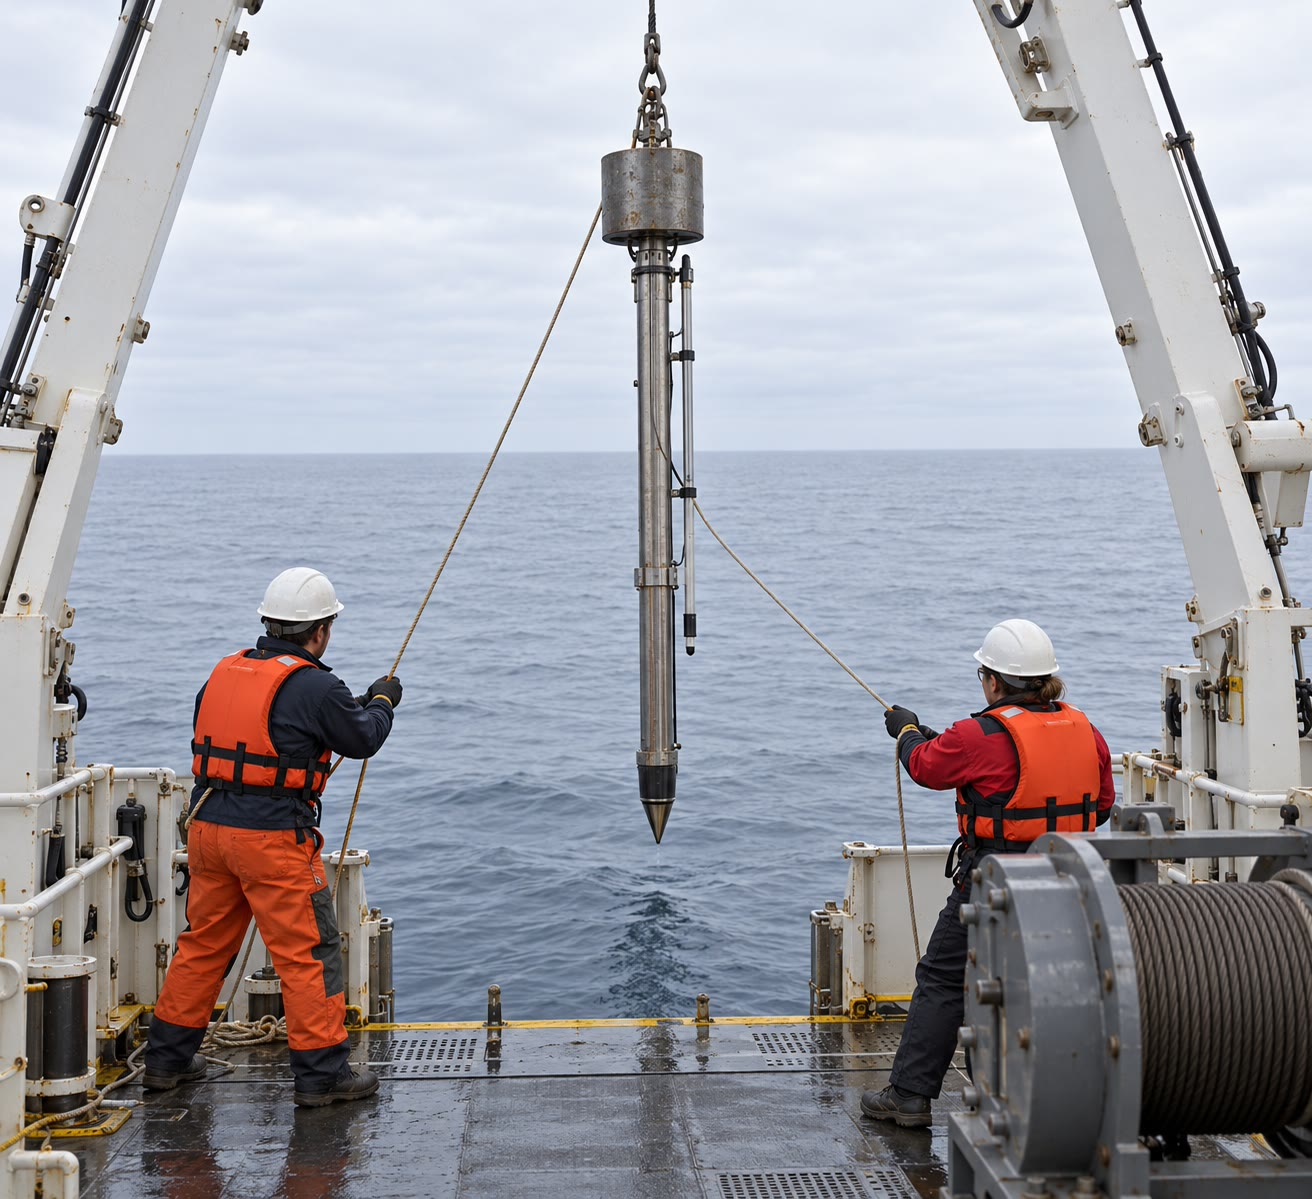
\includegraphics[width=\linewidth]{images/book5/ai/b3-heatflow-probe.jpg}

{\scriptsize Une lance à flux de chaleur sur le point d'être descendue depuis la poupe d'un
navire de recherche (illustration générée par IA).}
\end{minipage}
\end{inthefield}

\section{Exercices}

\begin{exercise}[$\star$]\label{exo:b3:lithosphere-thermal-models:1}
Avec $\kappa = \qty{e-6}{m^2.s^{-1}}$, calculer le temps conductif $L^2/\kappa$
pour $L = 1$, 10 et \qty{100}{km}, en millions d'années.
\end{exercise}

\begin{exercise}[$\star$]\label{exo:b3:lithosphere-thermal-models:2}
Une chaîne de montagnes subit une érosion de \qty{1}{mm/an}, et la roche remonte à travers
les \qty{30}{km} supérieurs de la croûte pour compenser cette perte. Avec $\kappa = \qty{e-6}{m^2.s^{-1}}$,
calculer le nombre de Péclet. Le géotherme de la chaîne peut-il être calculé par la seule
conduction~?
\end{exercise}

\begin{exercise}[$\star$]\label{exo:b3:lithosphere-thermal-models:3}
Dans le modèle du demi-espace ($T_0 = 0$, $T_m = \qty{1450}{\celsius}$, $\kappa =
\qty{0.8e-6}{m^2.s^{-1}}$), calculer la température à \qty{10}{km} sous le plancher
océanique âgé de \qty{5}{Ma} (\qty{1}{Ma} $= \qty{3.156e13}{s}$~; $\operatorname{erf}
0.445 = 0.471$).
\end{exercise}

\begin{exercise}[$\star$]\label{exo:b3:lithosphere-thermal-models:4}
Avec $C_q = \qty{490}{mW.m^{-2}.Ma^{1/2}}$, calculer le flux de chaleur à travers
un plancher océanique âgé de 1, 25 et \qty{100}{Ma}. Laquelle de ces trois valeurs
une sonde sous-estimerait-elle le plus probablement~?
\end{exercise}

\begin{exercise}[$\star\star$]\label{exo:b3:lithosphere-thermal-models:5}
Dans le modèle du demi-espace, la température atteint \qty{90}{\percent} de $T_m$
lorsque $\operatorname{erf}\eta = 0.9$, $\eta = 1.163$. Avec $\kappa =
\qty{0.8e-6}{m^2.s^{-1}}$, calculer cette profondeur pour \qty{10}{Ma}, \qty{40}{Ma} et \qty{100}{Ma}.
\end{exercise}

\begin{exercise}[$\star\star$]\label{exo:b3:lithosphere-thermal-models:6}
Avec les valeurs du texte, le modèle du demi-espace donne $C =
\qty{370.5}{m.Ma^{-1/2}}$. En gardant toutes les autres valeurs, quel coefficient de
dilatation thermique donnerait la valeur ajustée de \qty{350}{m.Ma^{-1/2}}~? Quel autre
paramètre pourrait être modifié à la place~?
\end{exercise}

\begin{exercise}[$\star\star$]\label{exo:b3:lithosphere-thermal-models:7}
Calculer le flux de chaleur asymptotique $kT_m/L$ du modèle de plaque pour $L =
\qty{95}{km}$, $T_m = \qty{1450}{\celsius}$, et pour $L = \qty{125}{km}$,
$T_m = \qty{1350}{\celsius}$, avec $k = \qty{3.1}{W.m^{-1}.K^{-1}}$ dans les deux cas.
Lequel est le plus proche du flux de chaleur d'un plancher océanique ancien calculé à partir de $C_q/\sqrt t$
à \qty{150}{Ma}, avec $C_q = \qty{490}{mW.m^{-2}.Ma^{1/2}}$~?
\end{exercise}

\begin{exercise}[$\star\star$]\label{exo:b3:lithosphere-thermal-models:8}
Une province présente $q_0 = \qty{60}{mW.m^{-2}}$, $h_r = \qty{10}{km}$ et $A_0h_r =
0.4\,q_0$. Calculer $A_0$, $q_m$ et la température au Moho, à \qty{35}{km}
de profondeur, avec $k = \qty{2.5}{W.m^{-1}.K^{-1}}$.
\end{exercise}

\begin{exercise}[$\star\star$]\label{exo:b3:lithosphere-thermal-models:9}
Deux plutons granitiques d'une même province donnent $q_0 = \qty{66}{mW.m^{-2}}$ avec $A_0
= \qty{3.0}{\micro W.m^{-3}}$, et $q_0 = \qty{48}{mW.m^{-2}}$ avec $A_0 =
\qty{1.2}{\micro W.m^{-3}}$. En supposant qu'ils se situent sur la droite de la
\cref{prop:b3:lithosphere-thermal-models:exponential}, calculer $h_r$ et $q_m$.
\end{exercise}

\begin{exercise}[$\star\star\star$]\label{exo:b3:lithosphere-thermal-models:10}
(a) Montrer que la chaleur perdue à travers le plancher océanique entre les âges 0 et $t$, par
unité de surface, vaut $Q(t) = 2k(T_m - T_0)\sqrt{t/(\pi\kappa)}$ dans le modèle du
demi-espace. (b) Montrer que la subsidence vaut $d - d_r = \alpha Q/\bigl(c(\rho_m -
\rho_w)\bigr)$, où $c = k/(\rho_m\kappa)$ est la chaleur massique. (c) Vérifier
numériquement ce résultat à \qty{40}{Ma} avec les valeurs du texte.
\end{exercise}

\begin{exercise}[$\star\star\star$]\label{exo:b3:lithosphere-thermal-models:11}
Dans le modèle de plaque du texte ($\tau = \qty{36.2}{Ma}$, $\rho_m\alpha T_mL/
\bigl(2(\rho_m - \rho_w)\bigr) = \qty{3104}{m}$), la profondeur calculée avec le seul
premier terme de Fourier dépasse la série complète principalement à cause du terme $n = 3$.
Calculer l'amplitude de ce terme à 1, 10 et \qty{20}{Ma}, ainsi que l'âge à partir duquel
le seul premier terme se situe à moins de \qty{10}{m} de la série.
\end{exercise}

\begin{exercise}[$\star\star\star$]\label{exo:b3:lithosphere-thermal-models:12}
(a) Montrer que, dans le géotherme de la \cref{prop:b3:lithosphere-thermal-models:exponential},
$T(z) \approx q_mz/k + A_0h_r^2/k$ pour $z \gg h_r$. (b) En déduire la profondeur de
l'isotherme de \qty{1300}{\celsius} pour $q_0 = \qty{40}{mW.m^{-2}}$, avec les valeurs
de l'exercice 8. (c) De combien $q_m$ doit-il diminuer pour que cette profondeur atteigne
\qty{250}{km}, profondeur des racines rapides des cratons~?
\end{exercise}

\section{Problème~: quarante millions d'années loin de la dorsale}

\begin{problem}[{Problème du week-end --- le demi-espace et la plaque, la profondeur d'un
océan inventé, et l'épaisseur de sa plaque}]
\label{pb:b3:lithosphere-thermal-models:1}
% values: calc/ch05.py; plate_cooling.py; honda04:gdh1, ps77:depth-age, data:b5-depth-age
Prendre $T_0 = 0$, $T_m = \qty{1450}{\celsius}$, $\kappa =
\qty{0.8e-6}{m^2.s^{-1}}$, $k = \qty{3.1}{W.m^{-1}.K^{-1}}$, $\alpha =
\qty{3.1e-5}{K^{-1}}$, $\rho_m = \qty{3300}{kg.m^{-3}}$, $\rho_w =
\qty{1030}{kg.m^{-3}}$, une dorsale profonde de \qty{2500}{m}, et \qty{1}{Ma} $=
\qty{3.156e13}{s}$.

\medskip\noindent\textbf{Partie I --- Le demi-espace.}
\begin{enumerate}
  \item Calculer $\sqrt{\kappa t}$ à 10 et \qty{40}{Ma}.
  \item Calculer la température à \qty{20}{km} sous le plancher aux deux âges
        ($\operatorname{erf}0.6294 = 0.6266$, $\operatorname{erf}0.3147 =
        0.3437$).
  \item L'isotherme de \qty{1000}{\celsius} se situe là où $\operatorname{erf}\eta =
        0.6897$, $\eta = 0.7174$. Calculer sa profondeur aux deux âges, ainsi que l'âge
        auquel elle atteint \qty{60}{km}.
  \item Calculer le flux de chaleur aux deux âges, ainsi que $C_q$.
  \item Une dorsale s'étale à \qty{25}{mm/an} de chaque côté. Calculer le nombre de Péclet
        de la plaque sur \qty{95}{km}. Pourquoi chaque colonne peut-elle être
        refroidie seule~?
  \item Calculer le temps conductif à travers \qty{95}{km}. Que dit-il d'un
        modèle de demi-espace pour un plancher âgé de \qty{150}{Ma}~?
\end{enumerate}

\medskip\noindent\textbf{Partie II --- Subsidence.}
\begin{enumerate}[resume]
  \item Rappeler l'équilibre isostatique qui transforme le déficit de température
        d'une colonne en subsidence, et pourquoi l'intégrale peut être prolongée à l'infini
        dans le demi-espace.
  \item Calculer $C$ de la loi profondeur--âge, ainsi que les profondeurs à 10 et
        \qty{40}{Ma}.
  \item La profondeur médiane du plancher océanique réel entre 40 et \qty{45}{Ma}
        est de \qty{4475}{m}, non corrigée. Comparer avec le modèle à
        \qty{42.5}{Ma}, et lister ce que la médiane inclut et que le modèle
        laisse de côté.
  \item De combien $C$ changerait-il si $T_m$ était de \qty{1350}{\celsius}~?
        Comparer avec la valeur ajustée de \qty{350}{m.Ma^{-1/2}}.
  \item Pourquoi les flux de chaleur mesurés sur un plancher jeune sont-ils inférieurs à $C_q/\sqrt t$~?
\end{enumerate}

\medskip\noindent\textbf{Partie III --- La plaque.} Prendre $L = \qty{95}{km}$.
\begin{enumerate}[resume]
  \item Calculer $\tau$ et l'amplitude $\rho_m\alpha T_mL/\bigl(2(\rho_m -
        \rho_w)\bigr)$.
  \item Calculer la profondeur à \qty{40}{Ma} avec les termes $n = 1$, 3 et 5.
  \item Quel écart le premier terme seul présente-t-il par rapport à ce résultat, et
        pourquoi si peu~?
  \item Calculer la différence entre le demi-espace et la plaque à \qty{40}{Ma} et
        \qty{50}{Ma}, puis estimer par interpolation linéaire l'âge auquel elle
        atteint \qty{100}{m}.
  \item Calculer le flux de chaleur de la plaque à \qty{40}{Ma}, avec les termes
        $n = 1$ à 3, et le comparer à celui du demi-espace.
  \item Donner la profondeur et le flux de chaleur asymptotiques.
\end{enumerate}

\medskip\noindent\textbf{Partie IV --- Un océan inventé.} Dans un océan inventé
dont la dorsale est à \qty{2500}{m} de profondeur, le plancher, une fois corrigé des
sédiments et à l'écart des monts sous-marins et des renflements, est à \qty{5700}{m} de profondeur à \qty{120}{Ma} et
\qty{4800}{m} à \qty{40}{Ma}. Le $L$ de la plaque est inconnu~; toutes les autres
valeurs sont celles données ci-dessus.
\begin{enumerate}[resume]
  \item En ne gardant que le premier terme de Fourier, écrire la profondeur à
        \qty{120}{Ma} en fonction de $L$, avec $\tau$ lui-même dépendant de
        $L$.
  \item Résoudre en $L$ par itération, en partant de $L = \qty{100}{km}$~: calculer
        $\tau$, puis le $L$ qui correspond à \qty{5700}{m} avec ce $\tau$, et
        recommencer.
  \item Avec le $L$ trouvé, calculer la profondeur à \qty{40}{Ma} et comparer
        avec le demi-espace et avec la valeur mesurée de \qty{4800}{m}.
  \item Calculer $\tau$ pour ce $L$, ainsi que la profondeur asymptotique de cet océan.
  \item À partir de quel âge le plancher se situe-t-il à moins de \qty{100}{m} de sa
        profondeur asymptotique~?
  \item Donner l'épaisseur $L$ de la plaque qui correspond au plancher âgé de l'océan
        inventé.
\end{enumerate}
\end{problem}
